
\documentclass[Recitation8_EU.tex]{subfiles}

\section{Expected Utility}

\begin{frame}{Oskar Morgenstern on John von Neumann}
	\begin{quote}
		Whenever Johnny saw a funny hat, he’d put [it] on…He had one with a little contraption that made a noise when you blew into it, and a light would flash at the same time. It was one of those children’s things, and he loved it.
	\end{quote}
\end{frame}

\begin{frame}{The hat picture}
\begin{figure}
	\centering
	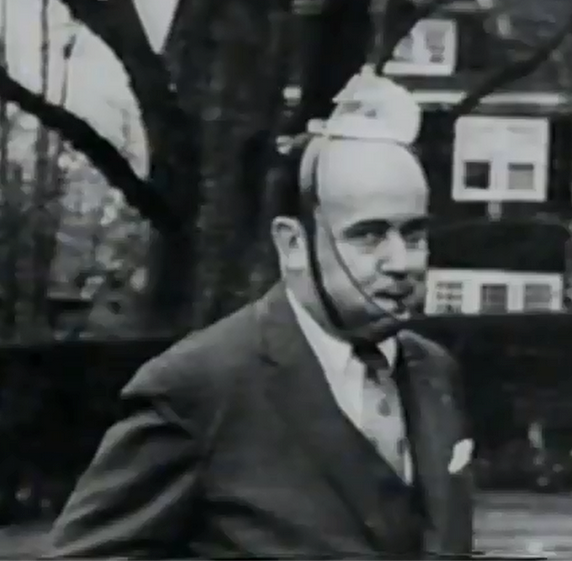
\includegraphics[width=0.6\linewidth]{Figures/vonneumann}
	\caption{}
	\label{fig:vonneumann}
\end{figure}
\end{frame}


\begin{frame}{A gamble and a poll}
	\begin{table}
		\centering
		\begin{tabular}{|c|c|c|c|}
			\multicolumn{2}{c}{\textbf{Experiment 1}} & \multicolumn{2}{c}{\textbf{Experiment 2}} \\
			\hline
			Gamble 1.A & Gamble 1.B & Gamble 2.A & Gamble 2.B\\
			\hline
			$\systeme*{&\$1m \ \text{w.p.} 1}$ &
			$\systeme*{&\$1m \ \text{w.p.} \ .89, &\$0 \ \text{w.p.} \ .01, &\$5m \ \text{w.p.} \ .10}$  & $\systeme*{&\$0 \ \text{w.p.} \ .89, &\$1m \ \text{w.p.} \ .11}$ & $\systeme*{&\$0 \ \text{w.p.} \ .90, &\$5m \ \text{w.p.} \ .10}$\\
			\hline
		\end{tabular}
	\end{table}

\end{frame}


\begin{frame}{Defining a Lottery}
	\begin{definition}
		A simple lottery $L$ is a list $L=\left(p_{1},...p_{N}\right)$ with
		$p_{n}\geq0$ for all $n$ and $\Sigma_{n}p_{n}=1,$ where $p_{n}$
		is interpreted as the probability of outcome $n$ occurring. 
	\end{definition}
Example:
\[
	\systeme*{x_1 = \$100 \ w.p. \ p_1 = .5, x_2 = \$200 \ w.p. \ p_2 = .5}
\]
Define the set of alternatives/gambles the
decision maker faces, denoted by $\mathcal{L}$, as the set of all simple
lotteries over possible outcomes $N$. How do we represent preferences on this set?\\
 In this class, \textbf{vNM}, which assumes that the agents have a  rational preference relation $\succsim$
 on $\mathcal{L}$, that for all $L\in\mathcal{L}$ can be represented as:
 \[
 	U(L) = \sum_{j=1}^{N}p_j u(x_j).
 \]
 These representation requires \textbf{two axioms} on preferences (we also assume completeness and transitivity).
 
\end{frame}


\begin{frame}{Axioms}
	 \textbf{Axiom 1. Continuity}\emph{. Small changes in probabilities
		do not change the nature of the ordering of two lotteries.}
	\vskip2ex
	\textbf{Axiom 2. Independence.} \emph{The preference relation }$\succsim$\emph{\ on
		the space of simple lotteries }$\mathcal{L}$\emph{ satisfies the independence
		axiom if for all }$L,L^{\prime},L^{\prime\prime}\in\mathcal{L}$\emph{
		and }$\alpha\in\left(0,1\right)$\emph{, we have} 
	\[
	L\succsim L^{\prime}\text{ if and only if ~}\alpha L+\left(1-\alpha\right)L^{\prime\prime}\succsim\alpha L^{\prime}+\left(1-\alpha\right)L^{\prime\prime}\text{. }
	\]
	Meaning:
	\begin{enumerate}
		\item Continuity: same as consumer theory. We can find a neighborhood in the space of lotteries where you prefer one lottery to another.
		\item Independence (from irrelevant alternatives) if you prefer a lottery to another, and I mix both of them up with another in the same proportion, you still satisfy the same ordering. The ``irrelevant alternative'' is the additional lottery $L''$ that I am mixing in
	\end{enumerate}
Are they reasonable?
\end{frame}

\begin{frame}{The vNM representation}
	
	\emph{The utility function }$U:\mathcal{L}\rightarrow\mathbb{R}$\emph{
		has an expected utility form if there is an assignment of numbers
	}$\left(u_{1},...u_{N}\right)$\emph{ to the }$N$\emph{ outcomes
		such that for every simple lottery }$L=\left(p_{1},...,p_{N}\right)\in\mathcal{L}$\emph{
		we have that }
	\[
	U\left(L\right)=u_{1}p_{1}+...+u_{N}p_{N}.
	\]
	In other words, a utility function has the expected utility form if
	and only if:
	\[
	U\left(\sum{}_{k=1}^{K}\alpha_{k}L_{k}\right)=\sum{}_{k=1}^{K}\alpha_{k}U\left(L_{k}\right)
	\]
	for any $K$ lotteries $L_{k}\in\mathcal{L}$, $k=1,...,K,$ and probabilities
	$\left(\alpha_{1},...,\alpha_{K}\right)\geq0$, $\Sigma_{k}\alpha_{k}=1.$ That is, the representation is linear in probabilities.\\
	\medskip
	\textbf{A utility function has the expected utility property
		if the utility of a lottery is simply the (probability-) weighted average
		of the utility of each of the outcomes.}
\end{frame}


\begin{frame}{Showing that the axioms imply vNM}
	\begin{theorem}
		 (Expected utility theory) Suppose that the rational preference
		relation $\succsim$ on the space of lotteries $\mathcal{L}$ satisfies
		the continuity and independence axioms. Then $\succsim$ admits a
		utility representation of the expected utility form. That is, we can
		assign a number $u_{n}$ to each outcome $n=1,...,N$ in such a manner
		that for any two lotteries $L=\left(p_{1},...,p_{N}\right)$ and
		$L^{\prime}=\left(p_{1}^{\prime},...p_{N}^{\prime}\right),$ we have
		$L\succsim L^{\prime}$ if and only if \[
		\sum\limits _{n=1}^{N}u_np_{n}\geq\sum\limits _{n=1}^{N}u_{n}p_{n}^{\prime}
		\].
	\end{theorem}
We will show that, under the two axioms, and for any two lotteries $L$ and $L'$, and $p\in
(0,1)$, there exists a utility function $U$ representing preferences
\textbf{over lotteries}, such that $U(p L + (1-p) L') = p U(L) +
(1-p) U(L')$. 
\end{frame}

\begin{frame}{Does it satisfy the axioms?}
\begin{itemize}
	\item  The definition of continuity would be something like: if there is a sequence of lotteries $\left\lbrace L_n\right \rbrace$, such that $L_n\succsim L''$ for all $n$, and the limit of the sequence is $L$, then $L\succsim L''$.\\
	\item Since the vNM function is linear, it is also a continuous function, and weak inequalities are preserved under the limit operator.
	\item Independence is very trivial: if you add something on both sides of the equal sign and multiply both sides by some number the inequality is preserved.
\end{itemize}

\end{frame}

\begin{frame}{Back to the Proof}
	We will show that, under the two axioms, and for any two lotteries $L$ and $L'$, and $p\in
	(0,1)$, we can build a utility function $U$ representing preferences
	\textbf{over lotteries}, such that $U(p L + (1-p) L') = p U(L) +
	(1-p) U(L')$. \\
	
	
	
	\begin{itemize}
		\item Step 1: Consider a fixed set of outcomes, and define $\overline{L}$ as the most-valued outcome and $\underline{L}$ as the least-valued. These outcomes are also \textit{degenerate lotteries}: we get an outcome with certain probability.
		\item Step 2: continuity implies that, for each outcome $L_i \in [\underline{L}, \overline{L}]$, there exists a probability $p_i\in (0,1)$ such that $p_i\overline{L} +(1-p_i)\underline{L} \sim L_i$.
		
	\end{itemize}
\end{frame}


\begin{frame}{Proof cont.}
\begin{itemize}
	\item Step 3: define the utility function $U(L_i)=p_i$ (the utility \emph{is the probability of the best outcome}, such that the mixture is indifferent to the lottery). Considering a lottery, $L_i$, we then have:
	\[
	L_i \sim p_i \overline{L} + (1-p_i)\underline{L} = U(L_i) \cdot \overline{L} + (1-U(L_i))\cdot\underline{L}
	\]
	
	\item The above represents the preferences, as a rational agent will prefer the lottery that gives the higher payoff with larger probability, therefore:
	\[
		L_1\succ L_2 \ {iff} \ U(L_1) = p_1>p_2 = U(p_2).
	\]
	\item Step 4: \textbf{by independence}, for any $p \in (0,1)$, the mixture:
	\[
		pL_1+(1-p)L_2 \sim p\left[p_1 \overline{L} + (1-p_1)\underline{L} \right] +(1-p) \left[p_2 \overline{L} + (1-p_2)\underline{L} \right]
	\]
\end{itemize}
That is:
\[
	U(pL_1 + (1-p)L_2) = pU(L_1) + (1-p)U(L_2).
\]

\end{frame}


\section{The Allais Paradox}

\begin{frame}{Allais ``Paradox''}
		\begin{table}
		\centering
		\begin{tabular}{|c|c|c|c|}
			\multicolumn{2}{c}{\textbf{Experiment 1}} & \multicolumn{2}{c}{\textbf{Experiment 2}} \\
			\hline
			Gamble 1.A & Gamble 1.B & Gamble 2.A & Gamble 2.B\\
			\hline
			$\systeme*{&\$1m \ \text{w.p.} 1}$ &
			$\systeme*{&\$1m \ \text{w.p.} \ .89, &\$0 \ \text{w.p.} \ .01, &\$5m \ \text{w.p.} \ .10}$  & $\systeme*{&\$0 \ \text{w.p.} \ .89, &\$1m \ \text{w.p.} \ .11}$ & $\systeme*{&\$0 \ \text{w.p.} \ .90, &\$5m \ \text{w.p.} \ .10}$\\
			\hline
		\end{tabular}
	\end{table}
If you choose 1.A and 2.B, your preferences are not vNM! They do not satisfy independence, as the above is the same as:
\begin{table}
	\centering
	\begin{tabular}{|c|c|c|c|}
		\multicolumn{2}{c}{\textbf{Experiment 1}} & \multicolumn{2}{c}{\textbf{Experiment 2}} \\
		\hline
		Gamble 1.A & Gamble 1.B & Gamble 2.A & Gamble 2.B\\
		\hline
		$\systeme*{&\$1m \ \text{w.p.} .89,&\$1m \ \text{w.p.} 11}$ &
		$\systeme*{&\$1m \ \text{w.p.} \ .89, &\$0 \ \text{w.p.} \ .01, &\$5m \ \text{w.p.} \ .10}$  & $\systeme*{&\$0 \ \text{w.p.} \ .89, &\$1m \ \text{w.p.} \ .11}$ & $\systeme*{&\$0 \ \text{w.p.} \ .89, &\$0 \ \text{w.p.} \ .01, &\$5m \ \text{w.p.} \ .10}$\\
		\hline
	\end{tabular}
\end{table}
Experiment 1 is just experiment 2, where in addition I give you a lottery where you win $\$1m$ in \textbf{both} scenarios. This should not flip your preferences according to vNM.
\end{frame}

